\documentclass[11pt, a4paper]{article}
\usepackage{polski}
\usepackage[utf8]{inputenc}
\usepackage{graphicx}
\usepackage{amsmath}
\usepackage{float}
\usepackage{multirow}
\usepackage{afterpage}
\usepackage{longtable}
\usepackage{makecell}
\usepackage{hyperref}
\usepackage{listings}
\usepackage[margin=1in]{geometry}
\usepackage{fancyhdr}
\usepackage{adjustbox}

\title{Metody głębokiego uczenia \\
Sprawozdanie z pierwszego projektu -- \\
Zaimplementowanie sieci MLP}
\author{Jadwiga Słowik, Paulina Tomaszewska}

\begin{document}
\maketitle
\section{Cel zadania}
Celem zadania było stworzenie sieci neuronowej, która~klasyfikuje obrazki z~ręcznie napisaną cyfrą do~kategorii odpowiadającej widocznej cyfrze.
Jako~zbiór danych posłużył zbiór~\textit{MNIST}, który~składa~się z~$60\:000$ obrazków treningowych i~$10\:000$~testowych. Rozmiar obrazków to~$28 \times 28$. Występują one jedynie w skali szarości, tzn. są zapisane w postaci jednej macierzy, a nie trzech jak w przypadku obrazków kolorowych (zapisanych w ramach konwencji RGB).

\section{Opis rozwiązania}
W~ramach projektu napisano w~języku \textit{Python} (przy~pomocy narzędzia \textit{jupyter-notebook}) sieć neuronową jednokierunkową -- \textit{MLP}.
Przy~konstruowaniu sieci skorzystano jedynie z~pakietów do~obliczeń macierzowych oraz~operacji na~ramkach danych (nie wykorzystano frameworków dedykowanym dziedzinie \textit{Deep Learning}): \textit{numpy} i~\textit{pandas}.

Rozwiązanie zadania składało~się z~następujących etapów:
\begin{enumerate}
    \item Wczytanie danych
    \item Przetworzenie danych (\textit{ang. preprocessing}) \\
    Dane zostały przetworzone w~celu zamiany wartości pikseli. Początkowo, wartości pikseli były liczbami naturalnymi z~przedziału $[0, 255]$. Docelowo, wartości pikseli zostały zmianione tak, by~były liczbami rzeczywistymi z~przedziału $[0, 1]$ -- normalizacja.
    \item Implementacja sieci \\
    Proces uczenia sieci neuronowej składa~się z~następujących etapów:
    \begin{enumerate}
        \item Inicjalizacja wag sieci losowymi wartościami
        \item Podział danych na~zbiór treningowy i~walidacyjny
        \item ,,Przetasowanie'' elementów zbioru treningowego
        \item Algorytm \textit{Feed-forward} dla~zbioru treningowego wraz z~obliczeniem funkcji kosztu \\
        Iteracyjnie, dla~kolejnych warstw sieci, obliczany jest wektor wartości wyjściowych (pojedynczy element wektora odpowiada wartości dla~odpowiedniego neuronu z~danej warstwy) korzystając z~następującego wzoru:
        \begin{equation}
            y = f\_activation_i(W_i \cdot x + b_i)
        \end{equation}
        $W_i$ to~macierz wag sieci neronowej (dla~$i$-tej warstwy), $x$ to~wektor wejść (wyniki dla~neuronów z~poprzedniej warstwy), $b_i$ -- wektor z~wartościami \textit{bias} dla~neuronów danej warstwy.
        
        W~naszym rozwiązaniu zaimplementowane zostały następujące funkcje aktywacji:
        \begin{equation}
            tanh(x) = \frac{e^x - e^{-x}}{e^x + e^{-x}}
        \end{equation}
        \begin{equation}
            sigmoid(x) = \frac{1}{1 + e^{-x}}
        \end{equation}
        \begin{equation}
            ReLU(x) = max(0, \, x)
        \end{equation}
        Ostatnia warstwa miała zawsze ustawioną funkcję aktywacji:
        \begin{equation}
            softmax(x) = \frac{e^x}{\sum_{i = 0}^{n - 1} e^{x_i}}\, , \quad \text{gdzie $n$ to długość wektora x}
        \end{equation}
        Ponadto, w~naszym rozwiązaniu zostały wykorzystane następujące funkcje kosztu (jako~$p$ (wektor ,,predykcji'') oznaczamy wektor z~wartościami prawdopodobieństw wystąpienia odpowiedniej klasy, natomiast~jako~$l$ oznaczamy klasę prawdziwą (oczekiwaną) przedstawioną w~formie \textit{one-hot-encoded}):
        \begin{equation}
            MSE(p,\, l) = \frac{\sum_{i=0}^{n-1} (p_i - l_i)^2}{n}
        \end{equation}
        \begin{equation}
            cross\_entropy(p, \, l) = -\sum_{i=0}^{n-1} l_i \cdot log(p_i + \epsilon)
        \end{equation}
        Dodanie $\epsilon$ do~wartości parametru logarytmu ma~na celu wyeliminowanie przypadku próby obliczenia logarytmu z~$0$. Jako $\epsilon$ wybraliśmy wartość $e^{-12}$. 
        
        \item Propagacja wsteczna przy~użyciu algorytmu \textit{SGD} (\textit{ang. Stochastic Gradient Descent}) \\
        Propagacja wsteczna jest wykonywana w~celu zaktualizowania wag sieci (oraz~wartości \textit{bias}) w~taki sposób, aby~uzyskać jak~najmniejszą wartość funkcji kosztu. Dlatego też, obliczany jest w~tym miejscu gradient funkcji kosztu, dzięki~któremu jesteśmy w~stanie określić kierunek najszybszego spadku wartości funkcji.
        
        Skorzystałyśmy z~następujących wzorów ([5]):
        \begin{equation}
            \delta^L = \nabla_a C \, \odot \, \sigma'(z^L)
        \end{equation}
        \begin{equation}
            \delta^l = ((W^{l+1})^T \, \delta^{l+1}) \, \odot \, \sigma'(z^l)
        \end{equation}
        \begin{equation}
            \frac{\partial C}{\partial b^l_j} = \delta_j^l
        \end{equation}
        \begin{equation}
            \frac{\partial C}{\partial w^l_{j,\,k}} = a_k^{l-1} \, \delta_j^l
        \end{equation}
        
        Wartości $a$ oznaczają kombinację liniową wag i~wejść do~neuronu powiększone o~\textit{bias}.
        
        Używając powyższych wzorów, jesteśmy w~stanie zaktualizować wartości wag (i~\textit{biasów}) w~sieci zgodnie z~następującymi wzorami:
        \begin{equation}
            w^l \rightarrow w^l - \frac{\eta}{m}\sum_x \delta^{x,l}(a^{x,l-1})^T
        \end{equation}
        \begin{equation}
            b^l \rightarrow b^l - \frac{\eta}{m}\sum_x\delta^{x,l}, \quad \text{gdzie $\eta$ to stała uczenia, $m$ -- rozmiar \textit{batcha}}
        \end{equation}
        
        \item Algorytm \textit{Feed-forward} (\textit{inference}) dla~zbioru walidacyjnego wraz z~obliczeniem funkcji kosztu
    \end{enumerate}
    Punkty \textit{(c) - (f)} powtarzamy tyle razy, ile~jest epok.
    
     Dokładniejszy opis zawarty jest w~punkcie dotyczącym \textit{ulepszeń podstawowego rozwiązania}.
    \item Testowanie przy użyciu wybranych hiperparametrów \\
    Proces predykcji klasy polega na~uruchomieniu funkcji \textit{Feed-forward} (\textit{inference}) dla~wytrenowanej sieci.
    
    Dokładniejszy opis procesu i~wyników testowania został zawarty w~rozdziale \textit{Wyniki}.
\end{enumerate}

\subsection{Architektura rozwiązania}
Sieć składa~się z kilku warstw. Pierwszą stanowi~warstwa wejściowa, która~wczytuje obrazki w~postaci wektorów $784$-elementowych
(każdy obrazek ze~zbioru ma~wymiary $28 \times 28$, co~daje łącznie $784$ piksele). Każdy~element wektora jest liczbą rzeczywistą należącą do~przedziału $[0, 1]$. Następnie są warstwy ukryte - gęste (\textit{ang. fully-connected}). Użytkownik może sam zdefiniować dla~każdej warstwy ukrytej liczbę neuronów a także jaką funkcję aktywacji chce użyć. Warstwa wyjściowa składa się z 10 neuronów - każdy odpowiada jednej z klas (tzn. odpowiedniej cyfrze). W przypadku tej warstwy została użyta funkcja \textit{softmax}, która~sprowadza wartości do~liczb z~przedziału $[0, 1]$, które sumują się do wartości 1. W~ten sposób modelujemy prawdopodobieństwo wystąpienia każdej z~klas.


\subsection{Ulepszenia podstawowego rozwiązania}
W~rozwiązaniu zastosowano następujące mechanizmy:
\begin{enumerate}
 \item Zbiór walidacyjny \\
 Wyodrębniono ze~zbioru treningowego zbiór walidacyjny ($10\:000$ elementów), który~w~oparciu o~metryki pozwalał na~lepsze analizowanie procesu uczenia~się sieci.
 Dzięki~temu rozwiązaniu możliwe jest zastosowanie np. \textit{kryterium stopu}, które w~sytuacji gdy~sieć zaczyna~się przeuczać (błąd~na~zbiorze walidacyjnym zaczyna gwałtownie rosnąć) zatrzymuje trening sieci i wraca do stanu wag sprzed wzrostu wartości błędów.
 
 
 \item Losowe tasowanie danych (\textit{shuffle}) \\
 Dane treningowe w~każdej epoce były poddawane losowemu przetasowaniu, tak~aby \textit{batche} w~każdej z~iteracji składały~się z~możliwie różnych~rekordów,
 co~zwiększa zdolność sieci do~generalizowania i~nieprzywiązywania~się do~kolejności wejściowych danych.
 
 \item Inicjalizacja wag \newline
 W przypadku nieprawidłowej inicjalizacji wag algorytm uczenia może nie zbiegać do rozwiązania, albo robić to wolniej niż w przypadku optymalnego doboru wartości początkowych. 
 Inicjalizacja wag w inny sposób niż poprzez zastosowanie wszędzie wartości zero nazywana jest \textit{złamaniem symetrii}. 
 Generalnie jeśli startowe wartości wag są za małe/duże może pojawić się problem \textit{vanishing/ exploding gradient}. Aby tego uniknąć a także przyspieszyć proces treningu sieci (znalezienia optimum) inicjalizuje się wartości wag z~rozkładu
 \(N(0,1/n_{in}))\). Inną często stosowaną metodą jest inicjalizacja Xaviera, zaproponowana przez Glorot \& Bengio [4]. Tą też metodę zaimplementowano w naszej sieci neuronowej typu MLP. 
  Wyróżnią się także metodę zwaną MSRA, która jest sugerowana w przypadku użycia w sieci funkcji aktywacji reLU.
 
  \item Optymalizator \newline
 W~rozwiązaniu zastosowano algorytm \textit{wstecznej propagacji} zwany \textit{Stochastic Gradient Descent (SGD)} z~uwzględnieniem podziału danych treningowych na~\textit{batche}.
 W~ten sposób nie~tylko proces uczenia przebiega efektywniej pod~względem wartości metryk, ale~też możliwe~są obliczenia macierzowe, które~pozwalają skrócić czas treningu sieci.
 
\textbf{Batch}\\
Zazwyczaj stosowanymi rozmiarami \textit{batchy} są: $32$, $64$, $128$, $256$ czy~$512$. W~naszym rozwiązaniu zdecydowałyśmy się na~$128$. Liczebność zbioru treningowego nie~stanowiła wielokrotności
wielkości rozmiaru \textit{batcha}, wówczas zdecydowano się, nie odrzucać pozostałych rekordów, tylko tworzyć mniej liczny \textit{batch}. Z uwagi na fakt, że zaakumulowane wartości gradientów wag były dzielone
przez~liczebność batcha, fakt, że jeden z nich był mniejszy nie~miał dużego znaczenia na~zbieżność algorytmu. 

\textbf{Regularyzacja wag}\\
W~celu uniknięcia sytuacji, gdy~wartości wag będą bardzo duże, zastosowano \textit{regularyzację} (nie~dotyczy to wag typu \textit{bias}). Wówczas, eliminuje się sytuację, gdy~mała różnica wartości na~wejściu powoduje duże różnice na~wyjściu sieci, co~sprawia, że~sieć traci zdolność generalizacji.

\textbf{Momentum}\\
W~algorytmie dano użytkownikowi możliwość treningu sieci z~uwzględnieniem \textit{momentum}.
Dzięki jego zastosowaniu trening jest bardziej stabilny (mniej ,,zygzakowaty''), ponieważ sieć zapamiętuje i~bierze pod~uwagę także kierunek zmian~wag (gradient wag) z~poprzedniej iteracji.

\item Data augmentation\newline
Technika \textit{data augmentation} jest często stosowana ze~względu na~dwa aspekty:
\begin{itemize}
 \item Zauważono, że sieci neuronowe wytrenowane na~małych zbiorach danych mają tendencję do~przeuczenia (\textit{overfitting}). [2] 
 \item Oczekuje się, aby~algorytmy klasyfikacyjne były~w~stanie wychwycić kluczowe cechy obrazków niezależnie od~skali, rozmiaru, lokalizacji, czy~kolorów obiektów na obrazkach (generalizacja).
\end{itemize}

W~ramach \textit{data augmentation} pewien reprezentatywny podzbiór danych treningowych (o~jednostajnym rozkładzie) poddawany jest transformacjom.
Stosuje się dwie klasy transformacji: geometryczne i fotometryczne.

W~ramach pierwszej grupy wyróżnia~się \textit{horizontal flipping},
rotację, losowe wycinanie (\textit{cropping}) itp. W ramach przekształceń fotometrycznych można modyfikować jasność, kontrast czy nasycenie kolorów.
Jedną z postawowych zasad, podczas stosowania \textit{data augmentation} jest konieczność zachowania pierwotnych etykiet danych.
Z~tego powodu w~przypadku zbioru \textit{MNIST} nie~można dokonywać transformacji \textit{horizontal flipping}.

\begin{figure}[H]
  \centering
  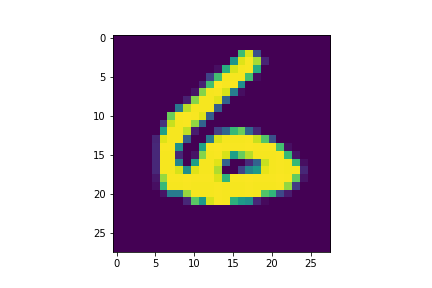
\includegraphics[scale=0.6]{original.png}
  \caption{Oryginalny obrazek}
\end{figure}

Jako transformacje zdefiniowano: 
\begin{itemize}
 \item przeskalowanie obrazka (i uzupełnienie zerami (\textit{padding}) do~rozmiaru obrazka wejściowego) \\
 \begin{figure}[H]
  \centering
  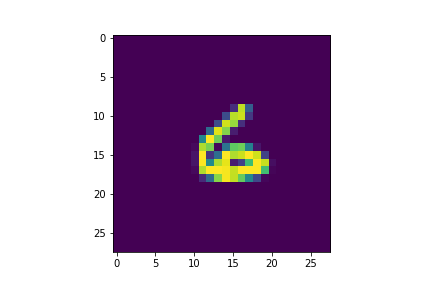
\includegraphics[scale=0.6]{rescaled.png}
  \caption{Obrazek przeskalowany}
 \end{figure}
 Miara przeskalowania jest generowana z~rozkładu jednostajnego z~przedziału $[0.5,\,\, 0.9]$ z~dokładnością do~jednego miejsca po~przecinku.
 \item rotację \\
 \begin{figure}[H]
  \centering
  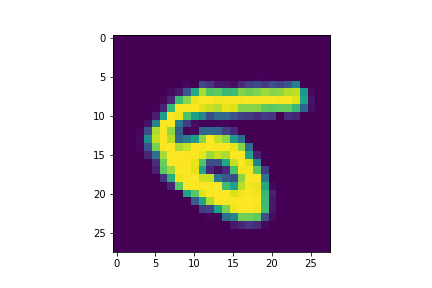
\includegraphics[scale=0.6]{rotated.png}
  \caption{Obrazek po zastosowaniu rotacji}
 \end{figure}
 Kąt rotacji generowany jest losowo z~rozkładu jednostajnego $[-40,\,\, 40]$ stopni.
 \item translację połączoną ze~zmniejszeniem ostrości obrazka \\
 \begin{figure}[H]
  \centering
  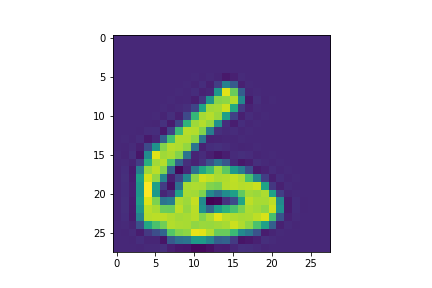
\includegraphics[scale=0.6]{translated1.png}
  \caption{Obrazek po translacji wraz~ze~zmniejszeniem ostrości}
 \end{figure}

 Wartości w~macierzy przesuwane są o~wektor, którego współrzędne pochodzą z~rozkładu jednostajnego $[-5,\,\, 5]$.
 Algorytm w~trakcie wykonywania tej operacji dokonuje pewnej interpolacji rzędu od~$0$ do~$5$. Im~wyższy jest~rząd, tym~obrazek jest~bardziej rozmyty
 (co~też stanowi użyteczną modyfikację w~kontekście \textit{data augmentation}), dlatego też rząd interpolacji również jest generowany z rozkładu jednostajnego.
 
 \item dodanie szumu \\
 \begin{figure}[H]
  \centering
  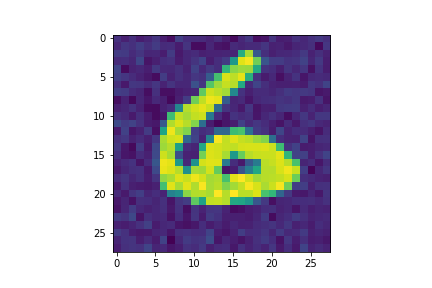
\includegraphics[scale=0.6]{noisy.png}
  \caption{Obrazek z dodanym szumem}
 \end{figure}

 Do~obrazków dodano szum z~rozkładu gaussa o~parametrach (średnia = $0$, odchylenie standardowe = $0.05$)
 
 \item \textit{ZCA whitening} (wybielanie) \\
 \begin{figure}[H]
  \centering
  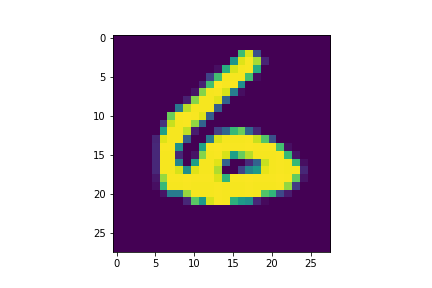
\includegraphics[scale=0.6]{zca.png}
  \caption{Obrazek po zastosowaniu mechanizmu wybielania}
 \end{figure}

 Metoda polegająca na~ekstrakcji poprzez~rozkład według~wartości osobliwych (\textit{SVD}) macierzy charakteryzujących konkretny rekord, aby~na~ich podstawie wyliczyć macierz przekształcenia
 (w~tej~metodzie nie~ma losowości).
 
\textit{ZCA whitening} [1] jest~liniową transformacją, która~randomizuje wejściowy wektor:
\begin{equation}
 x=\left(x_1,\ x_2,\ \ldots,\ x_n\right)
\end{equation}
poprzez~wykorzystanie macierzy~kowariancji:
\begin{equation}
 cov\left(x\right)=\ \mathrm{\Sigma}
\end{equation}
w ramach wyrażenia: \\
\begin{equation}
 y = (y_1,\, y_2, \, \ldots,\, y_n)^T \: \: = \: \: W \cdot x
\end{equation}

z~zachowaniem własności, że:
\begin{equation}
 cov\left(y\right)=I
\end{equation}
Macierz~$W$ nazywana jest~\textit{whitening matrix} i~musi spełniać warunek:
\begin{equation}
 W^T \cdot W \: \: = \: \: \Sigma^{-1}
\end{equation}
W~przypadku tego przekształcenia zmiany nie~są widoczne ,,gołym okiem''.
\end{itemize}
\end{enumerate}

\section {Szczegóły implementacyjne}
Użytkownik może zdefiniować sam konkretną topologię sieci (liczbę warstw ukrytych oraz~liczbę neuronów na~każdej warstwie) oraz następujące parametry:
\begin{itemize}
    \item funkcje aktywacji dla~każdej warstwy ukrytej (do~wybou: \textit{tanh}, \textit{sigmoid}, \textit{ReLU})
    \item funkcja kosztu (do~wyboru: \textit{cross-entropy}, \textit{mse})
    \item regularyzacja
    \item \textit{weight decay}
    \item \textit{momentum}
    \item rozmiar \textit{batcha}
    \item współczynnik uczenia (\textit{ang. learning rate})
    \item liczba epok
\end{itemize}
\section {Wyniki}
W~celu porównania efektywności i~poprawności sieci z~różnymi parametrami napisano skrypt do~automatycznych testów, który zbierał metryki w~postaci \textit{accuracy} do~pliku w~formacie \textit{JSON}.
Następnie w~skrypcie \texttt{tests\_analysis.ipynb} dokonano zestawienia wyników.
 
We wszystkich testach zgromadzonych w~zestawieniu poniżej użyto \textit{learning rate} o~wartości $0.04$, \texttt{batch\_size} równy $128$,
\textit{weight decay} równy~$0.005$ oraz~momentum o~wartości~$0.9$.

\begin{center}
    \begin{adjustbox}{angle=90}
    \begin{tabular}{lrrllllll}
    \hline
   \textbf{id} & \textbf{accuracy} & \textbf{epochs} & \textbf{error\_function} & \textbf{hidden\_activ\_func} & \textbf{hidden\_layer\_num} & \textbf{img\_augme} & \textbf{momentum} & \textbf{regularization} \\
    \hline 
    30 & 0.9744 & 30 & cross\_entropy & [relu] * 2 & [128] * 2 & True & False & False \\
    21 & 0.9727 & 20 & cross\_entropy & [tanh] * 3 & [128] * 3 & True & False & False \\ 
    1 & 0.9715 & 30 & cross\_entropy & [tanh] * 4 & [128] * 4 & False & True & False \\ 
    16 & 0.9701 & 20 & cross\_entropy & [relu] * 2 & [128] * 2 & False & False & False \\ 
    0 & 0.9695 & 30 & cross\_entropy & [tanh] * 2 & [128] * 2 & False & True & False \\ 
    20 & 0.9692 & 20 & cross\_entropy & [tanh] * 3 & [128] * 3 & False & False & False \\ 
    12 & 0.9686 & 20 & cross\_entropy & [tanh] * 2 & [128] * 2 & False & False & False \\ 
    17 & 0.9684 & 20 & cross\_entropy & [relu] * 2 & [128] * 2 & True & False & False \\ 
    26 & 0.9682 & 20 & cross\_entropy & [tanh] * 2 & [128] * 2 & False & True & False \\ 
    4 & 0.9681 & 20 & cross\_entropy & [tanh] * 2 & [128] * 2 & False & True & False \\ 
    24 & 0.9666 & 20 & cross\_entropy & [tanh] * 2 & [128] * 2 & True & False & False \\ 
    31 & 0.9665 & 20 & cross\_entropy & [tanh] * 5 & [128, 64, 32, 16, 8] & True & False & False \\ 
    13 & 0.9659 & 20 & cross\_entropy & [tanh] * 2 & [128] * 2 & True & False & False \\ 
    19 & 0.9600 & 20 & cross\_entropy & [tanh] * 1 & [128] * 1 & True & False & False \\ 
    28 & 0.9592 & 20 & cross\_entropy & [tanh] * 3 & [128] * 3 & True & True & True \\ 
    18 & 0.9579 & 20 & cross\_entropy & [tanh] * 1 & [128] * 1 & False & False & False \\ 
    10 & 0.9571 & 10 & cross\_entropy & [tanh] * 2 & [128] * 2 & False & False & False \\ 
    27 & 0.9536 & 20 & cross\_entropy & [tanh] * 2 & [128] * 2 & True & True & True \\ 
    5 & 0.9519 & 20 & cross\_entropy & [tanh] * 10 & [20] * 10 & False & True & False \\ 
    25 & 0.9514 & 20 & cross\_entropy & [tanh] * 2 & [128] * 2 & False & False & True \\ 
    8 & 0.9510 & 20 & cross\_entropy & [tanh] * 5 & [20] * 5 & True & True & True \\ 
    2 & 0.9504 & 30 & cross\_entropy & [tanh] * 2 & [20] * 2 & False & True & False \\ 
    3 & 0.9498 & 20 & cross\_entropy & [tanh] * 5 & [20] * 5 & False & True & False \\ 
    6 & 0.9368 & 20 & cross\_entropy & [tanh] * 20 & [20] * 20 & False & True & False \\ 
    15 & 0.9220 & 20 & cross\_entropy & [sigmoid] * 2 & [128] * 2 & True & False & False \\ 
    14 & 0.9205 & 20 & cross\_entropy & [sigmoid] * 2 & [128] * 2 & False & False & False \\ 
    11 & 0.8842 & 5 & cross\_entropy & [sigmoid] * 2 & [128] * 2 & True & False & False \\ 
    9 & 0.3596 & 5 & mse & [tanh] * 2 & [128] * 2 & False & False & False \\ 
    22 & 0.3387 & 20 & mse & [tanh] * 2 & [128] * 2 & False & False & False \\ 
    29 & 0.3167 & 20 & mse & [tanh] * 2 & [128] * 2 & False & True & False \\ 
    23 & 0.2888 & 20 & mse & [tanh] * 2 & [128] * 2 & True & False & False \\ 
    7 & 0.2110 & 20 & cross\_entropy & [tanh] * 30 & [20] * 30 & False & True & False \\ 
    \end{tabular}
 \end{adjustbox}     
\end{center}
\newpage
 Najlepszą siecią w~naszym przypadku ($97.44\%$) okazała~się sieć z~dwoma warstwami ukrytymi z~$128$ neuronami w~każdej i~funkcjami aktywacji w~postaci reLU. Sieć była trenowana przez~$30$ epok, a~zbiór treningowy został powiększony o~$1000$ obrazków w~ramach \textit{data augmentation}. Niewiele gorszym wskaźnikiem \textit{accuracy} skutkowało zastosowanie sieci z~trzema warstwami ukrytymi ($128$ neuronów w~każdej) z~funkcjami aktywacji \textit{tanh} trenowana przez~\textit{20} epok ($97.27\%$). W~tym wypadku także zastosowano \textit{data augmentation}.
 
 \subsection {Wpływ parametrów sieci na wartosć \textit{accuracy}}
 Poniżej zostało przedstawione, jaki~wpływ na~wartość \textit{accuracy} ma~dobór odpowiednich parametrów sieci.
 \subsubsection{Wpływ różnych funkcji aktywacji}
 Testy o~identyfikatorach $16$ i~$12$ różniły~się jedynie rodzajem zastosowanych funkcji aktywacji
 W~sieci o~numerze $16$ zastosowano we~wszystkich warstwach \textit{reLU}, natomiast w~$12$ -- tangens hiperboliczny.
 Okazało~się, że~w~przypadku zastosowania funkcji \textit{reLU} wartość \textit{accuracy} była o~$0.15$ pkt. procentowego wyższa niż~w~przypadku funkcji~\textit{tanh}.
 Można więc stwierdzić, że~różnica jest~znikoma. Analogiczny test ($14$) został przeprowadzony dla~sieci o~takich samych parametrach jednak z~funkcją aktywacyjną \textit{sigmoid}.
 W~tym przypadku \textit{accuracy} było aż o~$4.96$ pkt. procentowego niż~dla analogicznej sieci z~funkcją \textit{reLU}. 
 
W~zaimplementowanej przez~nas sieci neuronowej funkcja \textit{sigmoid} skutkuje znacznie mniejszą wartością \textit{accuracy} niż~\textit{reLU} i~\textit{tanh}.
 
 \subsubsection{Wpływ zastosowania w algorytmie SGD momentum}
 Porównując testy z tabeli o~oznaczeniach $12$ i~$26$, można~stwierdzić, że~różnią~się jedynie~tym, że~w~przypadku testu~$26$ zastosowano \textit{momentum}. 
 Sieć była trenowana przez~$20$ epok, używając jako~funkcji kosztu \textit{cross entropy}. Składała~się z~dwóch warstw ukrytych o~$128$ neuronach.
 Użyto funkcji aktywacji \textit{tanh}. 
 Okazało~się, że~w~przypadku użycia \textit{momentum} (test $26$) sieć osiągnęła minimalnie wyższe (o $0.04$ pkt. procentowego) \textit{accuracy}.
 Niemniej jest to wielkość tak mała, że~można uznać, iż~w~tym~konkretnym przypadku wpływ zastosowania w~sieci \textit{momentum} na~poprawność klasyfikacji jest znikomy. 
 
 \subsubsection{Wpływ zastosowania data augmentation} 
 Testy o numerach $20$ i~$21$ różnią~się jedynie~tym, w~pierwszym przypadku zastosowano \textit{data augmentation}. Ta~też sieć skutkowała \textit{accuracy} lepszym o~$0.35$ pkt. proc.
 Warto podkreślić, że~w~ramach \textit{data augmentation} zmodyfikowano jedynie $1\:000$ obrazków (ze względu na~zasoby obliczeniowe).
 W~przypadku większego odsetka przekształconych obrazków, można by było oczekiwać większej poprawy \textit{accuracy}.
 
 \subsubsection{Wpływ regularyzacji}
 Testy o numerach $25$ i~$12$ różnią~się jedynie~tym, że~w~przypadku tego~pierwszego zastosowano \textit{regularyzację}.
 Niemniej okazało się, że~zastosowanie czynnika \textit{weigth decay} pogorszyło zdolność sieci do~poprawnej klasyfikacji o~$1.72$ pkt. procentowego.
 
 \subsubsection{Wpływ liczby epok}

Porównano wynik błędu klasyfikacji dla~sieci z~dwoma warstwami ukrytymi ($128$ neuronów w~każdej warstwie) z~funkcjami aktywacji -- \textit{tanh},
bez zastosowania \textit{regularyzacji}, \textit{momentum}, ani~\textit{data augmentation} dla~różnej liczby epok treningowych.
\begin{figure}[H]
 \centering
 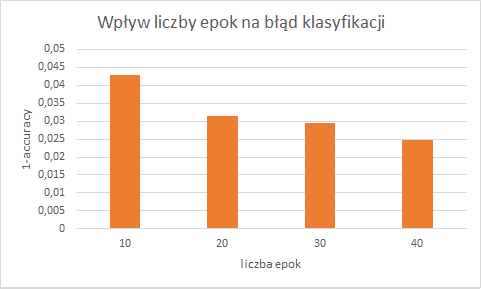
\includegraphics[scale=0.8]{epoki_nn.png}
 \caption{Wykres porównujący wartość \textit{accuracy} ze~względu na~liczbę epok}
\end{figure}

Wyraźnie widać, że~dla analizowanej architektury trend jest spadkowy, czyli~im więcej epok tym mniejszy błąd klasyfikacji.


 \subsubsection{Wpływ liczby warstw}
 Analizowane architektury sieci miały po~$20$ neuronów w~warstwach ukrytych. Jako~funkcji aktywacji użyto~\textit{tanh}. Sieci byłby trenowane prze~$20$ epok -- z~wykorzystaniem \textit{momentum}.
 \begin{figure}[H]
  \centering
  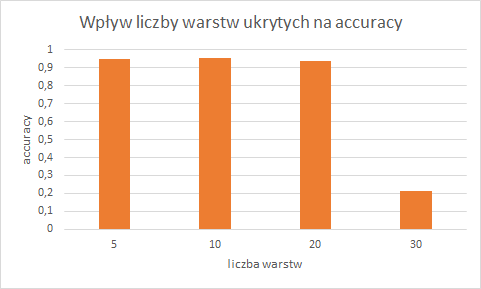
\includegraphics[scale=0.8]{warstwy_nn.png}
  \caption{Wykres porównujący wartość \textit{accuracy} ze~względu na~liczbę warstw}
 \end{figure}

Można zaobserwować, że~użycie $5$, $10$, $20$~warstw ukrytych skutkowało ponad $90\%$ \textit{accuracy}, podczas~gdy zastosowanie $30$~warstw wiązało~się z~dużym spadkiem
poprawności klasyfikacji do~wartości jedynie ok. $20\%$.  
 
 \subsubsection{Wpływ liczby neuronów}
 Porównano sieć o~identyfikatorach równych $2$ i~$26$. Obie byłby trenowane przez~$20$~epok z~zastosowaniem \textit{momentum}.
 Pierwsza z~nich miała dwie warstwy ukryte składające~się z~$20$~neuronów, natomiast druga -- $128$ neuronów. Mniejsza sieć cechowała się gorszą o $1.78$ pkt. wartością \textit{accuracy}.
 
 \bigbreak
 W następnych podrozdziałach zaprezentowano szczegółowe wartości metryk dla sieci, która skutkowała najlepszą wartością accuracy.
 \subsection{Wykres \textit{ROC}}
 Poniżej został przedstawiony wykres \textit{ROC}, na~który zostały nałożone dane dotyczące każdej klasy.
 Oddzielne wykresy dla~każdej z~klas zostały zawarte w~pliku \texttt{tests\_analysis.ipynb}.
 Na wykresie poniżej widać, że dla każdej z kategorii pole powierzchni pod krzywą ROC wynosi niemal wartość maksymalną równą 1 (która odpowiada idealnym klasyfikatorom). Warto też podkreślić, że kształt krzywych ROC jest praktycznie linią prostą (nie jest poszarpana). 
 \begin{figure}[H]
		\centering
		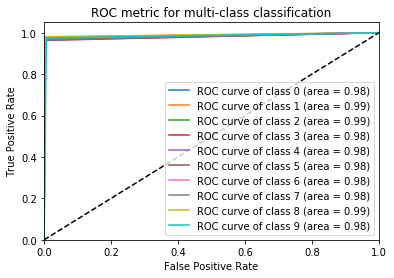
\includegraphics[scale=0.5]{roc_auc.png}
		\caption{Wykres ROC dla wszystkich klas}
\end{figure}
	
\subsection{Macierz pomyłek}
Poniżej została przedstawiona macierz pomyłek dla ,,najlepszej'' sieci
\begin{figure}[H]
		\centering
		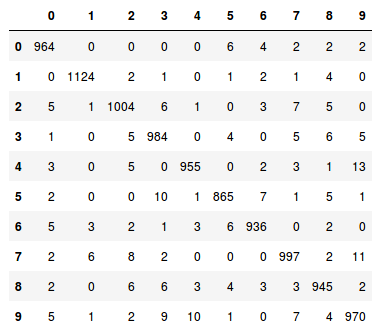
\includegraphics[scale=0.5]{conf_matrix.png}
		\caption{Macierz pomyłek dla ,,najlepszej'' sieci}
\end{figure}
Można wywnioskować, że~najwięcej pomyłek było przy~próbie klasyfikacji obrazka, na~którym była zapisana czwórka i~został on zaklasyfikowany jako~dziewiątka ($13$ błędów tego rodzaju). Również, w~odwrotny sposób -- klasyfikator $10$ razy sklasyfikował dziewiątkę jako~czwórkę.

\subsection{Raport klasyfikacji}
Poniżej znajdują~się obliczone metryki \textit{precision}, \textit{recall} oraz~\textit{f1} dla~każdej klasy osobno. Wyniki zostały sporządzone w~oparciu o~sieć dającą najwyższe \textit{accuracy}.

\begin{table}[H]
		\centering
    \begin{tabular}{llll}
    \textbf{klasa} & \textbf{precision} & \textbf{recall} & \textbf{f1} \\
    \hline
     0 & 0.97 &     0.98  &    0.98     \\
        1 &      0.99 &     0.99 &     0.99  \\
        2 &      0.97 &     0.97 &     0.97  \\
        3 &      0.97 &     0.97 &     0.97 \\ 
        4 &      0.98 &     0.97 &     0.98 \\
        5 &      0.98 &     0.97 &     0.97  \\ 
        6 &      0.98 &     0.98 &     0.98  \\ 
        7 &      0.97 &     0.97 &     0.97  \\ 
        8 &      0.97 &     0.97 &     0.97  \\ 
        9 &      0.97 &     0.96 &     0.96  \\
    \end{tabular}
    \caption{Raport klasyfikacji dla ,,najlepszej'' sieci}
\end{table}

\subsection{Wykresy funkcji kosztu}
Poniżej przedstawiono wykres funkcji kosztu dla~sieci uzyskującej najwyższe \textit{accuracy}. Wyraźnie widać, że wartości obu funkcji maleją, a więc nie występuje zjawisko przeuczenia.
\begin{figure}[H]
    \centering
    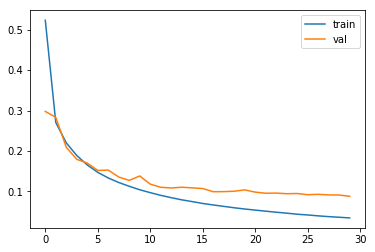
\includegraphics[scale=0.7]{funkcja_kosztu.png}
    \caption{Wykres funkcji kosztu dla sieci o~najwyższym \textit{accuracy}}
\end{figure}

Wykresy funkcji kosztu dla~innych sieci zostały zamieszczone w~\textit{notebooku} z~zawartym kodem i~procedurą testowania sieci.

\subsection{Źle sklasyfikowane obrazki}
Sieć o~największym \textit{accuracy} sklasyfikowała niepoprawnie łącznie $256$~obrazków.
Wykaz wszystkich obrazków został zawarty w~pliku \texttt{tests\_analysis.ipynb}. Poniżej~znajduje~się
kilka wybranych przykładów.

 \begin{figure}[H]
		\centering
		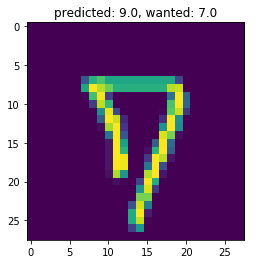
\includegraphics[scale=0.5]{wrong_class_0.png}
		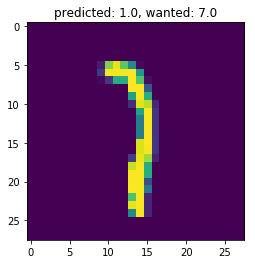
\includegraphics[scale=0.5]{wrong_class_1.png}
		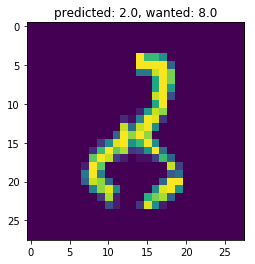
\includegraphics[scale=0.5]{wrong_class_2.png}
		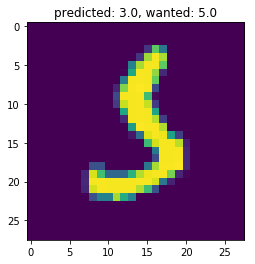
\includegraphics[scale=0.5]{wrong_class_3.png}
		\caption{Wybrane źle sklasyfikowane obrazki przez~,,najlepszą'' sieć}
\end{figure}


 \section {Wnioski}
 Na podstawie analizy wyników uzyskanych przez~różne topologie sieci neuronowych zauważono, że $30$-sto czy~$5$-cio warstwowe skutkowały znacznie mniejszym \textit{accuracy}
 niż~sieci płytkie. Podejrzewa~się, że~wynika~to z~wystąpienia zjawiska \textit{vanishing gradient}, który~polega na~tym, że~w~trakcie propagacji~wstecznej przez~wiele warstw
 wielokrotnie mnoży~się gradienty o~małych (często mniejszych od zera wartości), co powoduje, że~dążą one do~zera. Natomiast, w~sytuacji, gdy~gradienty są~zerowe sieć przestaje
 mieć zdolność do~aktualizacji wag w~danej warstwie, a~więc proces uczenia znacznie ,,wyhamowywuje''. 
 
Zdecydowanie niższą wartością \textit{accuracy} skutkowało użycie jako~funkcji kosztu -- \textit{MSE}. Wynik ten pokrywa~się z~przewidywaniami, bowiem~\textit{MSE}
jest zazwyczaj stosowane w~zadaniu regresji, natomiast \textit{cross entropy} w~zadaniach~klasyfikacji. 


 
 \section {Możliwe kierunki rozwoju projektu}
 Na~\textit{perfomance} sieci neuronowej wpływa wiele czynników. Jedną z~kluczowych decyzji jest wybór optymalizatora. W~naszym rozwiązaniu
 zastosowano algorytm \textit{SGD}, niemniej warto by~było przetestować jeszcze algorytm \textit{Adam} czy~\textit{RMSProp},
 które~z~uwagi na~bardziej wyszukane formuły pozwalają na~efektywniejszy trening sieci. W~przypadku zastosowania algorytmu \textit{Adam} mniej istotny staje~się dobór
 hiperparametru \textit{learning rate}, ponieważ~jego wartość jest dostosowywana na~bieżąco na~podstawie przebiegu procesu uczenia. 
 Warto także także wzbogacić algorytm o~kryterium stopu, które~w~sytuacji gwałtownego wzrostu błędu (np. trzykrotnego) na~zbiorze walidacyjnym zakończy trening i~wróci do~poprzedniego stanu wag,
 takie rozwiązanie wymagałoby przechowywania w~ramach działania programu w~każdej iteracji zestawu wag z~poprzedniej epoki.
 
 Ciekawym zagadnieniem byłoby także zastosowanie \textit{data augmentation} w~postaci \textit{elastic transformation} [3]. W~ramach tego przekształcenia symuluje~się efekty wynikająca z~różnych skurczy mięśni dłoni. Transformacja ma charakter dwuparametrowy \((\alpha, \sigma)\). Pierwszy z~nich określa miarę zniekształcenia, natomiast drugi ,,gładkość'' transforamacji. Poniżej zaprezentowano porównanie obrazków przed i po zastosowaniu transformacji.\newline
 
 \begin{figure}[H]
  \centering
    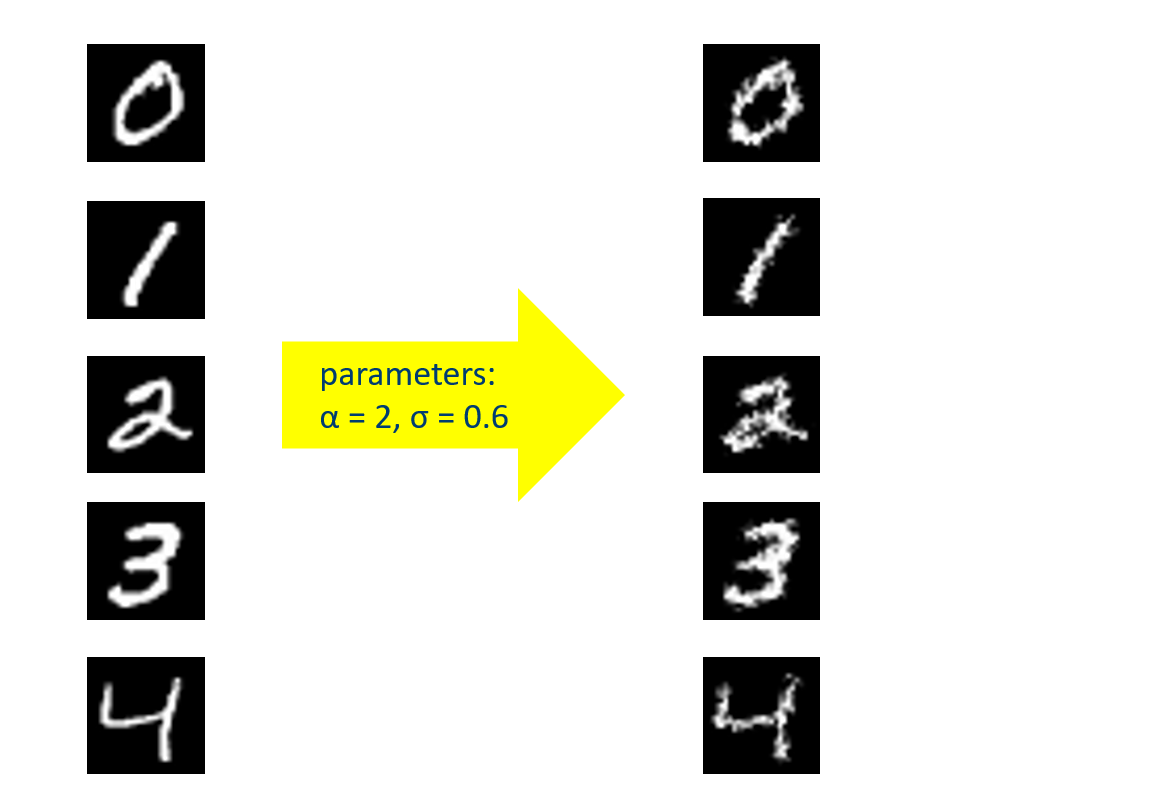
\includegraphics[scale=0.5]{elastic_transformation.png}
    \caption{\textit{Elastic transformation}, Opracowanie własne}
 \end{figure}

\section{Bibliografia}
[1] Agnan Kessy, Alex Lewin, Korbinian Strimmer, ‘Optimal whitening and decorrelation’, 2016 \newline
[2] Christopher M. Bishop, ‘Pattern Recognition and Machine Learning (Information Science and Statistics)’, 2006 \newline
[3] Partice Y. Simard, Dave Steinkraus, John C. Platt, ‘Best practices for convolutional neural networks applied to visual document analysis’, 2003 \newline
[4] Xavier Glorot and Yoshua Bengio, chapter: Understanding the difficulty of training neural networks, 'Proceedings of the Thirteenth International Conference n Artificial Intelligence and Statistics', pages 249-256; 2010 \newline
[5] http://neuralnetworksanddeeplearning.com


\end{document}